\documentclass{beamer}

\beamertemplatenavigationsymbolsempty

\usepackage{fontspec}
\usepackage{pgfpages}
\usepackage{tikz}
\usetikzlibrary{arrows}
\usetikzlibrary{shapes.misc}
\tikzset{
  invisible/.style={opacity=0},
  visible on/.style={alt={#1{}{invisible}}},
  alt/.code args={<#1>#2#3}{%
    \alt<#1>{\pgfkeysalso{#2}}{\pgfkeysalso{#3}} % \pgfkeysalso doesn't change the path
  },
}

\setbeameroption{show notes}
\setbeameroption{show notes on second screen=right}

\setsansfont{Josefin Sans}
\setmainfont{Josefin Slab}

\definecolor{gitcol}{HTML}{F05033}
\definecolor{bashbkg}{HTML}{111111}
\setbeamercolor{structure}{fg=gitcol}
\setbeamertemplate{navigation symbols}{}

\usetheme{Bergen}

\title{Git Distributed Version Control}
\author{Louis Burke}
\logo{\includegraphics[scale=0.1]{GitIcon}}

\begin{document}

\frame{\titlepage}

\begin{frame}{What is Version Control?}

    \begin{itemize}
        \item<1->Keeping track of multiple versions

        \item<2->Enabling collaboration

        \item<3->Examples?
    \end{itemize}

    \note<1>{System for keeping track of project versions}

    \note<2>{Distributed collaboration}

    \note<3>{Non-vcs. e.g.: file1, file2, file2.1 / google docs}
\end{frame}

\begin{frame}[fragile]{What is Git?}
    \begin{verbatim}
$ git gud
git: 'gud' is not a git command. See 'git --help'.

The most similar command is
        gui
    \end{verbatim}
    \begin{itemize}
        \item<2->Distributed Version Control

        \item<3->Created for the Linux Kernel

        \item<4->Most widely used VCS

        \item<5->Hosting services
            \begin{itemize}
                \item<5->Github
                \item<5->Bitbucket
                \item<5->Gitlab
            \end{itemize}
    \end{itemize}

    \note<2>{Git is ... unlike many other versions, no central repo required
    (not server-client)}

    \note<3>{By Linus Torvalds, currently maintained by Junio Hamano (Google)}

    \note<4>{VCS = version control system ... This means most professional
    programmers are familiar with it.}

    \note<5>{Also has many free hosting services. They provide a remote server
    that can be used.}
\end{frame}

\begin{frame}{Benefits}
    \begin{itemize}
        \item<1->Easy to use*

        \item<2->Powerful

        \item<3->Fast

        \item<4->Lightweight
    \end{itemize}

    \note<1>{Relative to some common alternatives, once learned.}

    \note<2>{Graph theory}

    \note<3>{Written in C, etc}

    \note<4>{Saves patches as diffs instead of full copies}
\end{frame}

\begin{frame}{Basics}
    \begin{itemize}
        \item<1->Repository (AKA "repo")

        \item<2->Commits

        \item<3->Branches

        \item<4->Remotes
    \end{itemize}

    \note<1>{The entire project + tracking info is called a repo.}

    \note<2>{Repo made up of many commits = diff of files}

    \note<3>{Branches keep track of commits}

    \note<4>{Branches on other computers are "remote" but can still be accessed}
\end{frame}

\begin{frame}{Saving}
    \begin{itemize}
        \item<1->Save file

        \item<2->Staging area

        \item<3->Committed

        \item<4->Pushed*
    \end{itemize}

    \note<1>{When you save a file, its just saved.}

    \note<2>{Then you add to repo by 'staging' it.}

    \note<3>{Then you commit the staging area to create a new commit.}

    \note<4>{Then you might push that commit to some remote server for safe
    storage.}
\end{frame}

\begin{frame}{Branching}
    \begin{itemize}
        \item<1->Lets you 'split'

        \item<2->Starts with 'master' (usually)

        \item<3->Need merging...
    \end{itemize}

    \note<1>{Branches let you switch between different changes/features}

    \note<2>{Most repos start with a 'master' branch}

    \note<3>{Bringing branches together can be tricky}
\end{frame}

\begin{frame}{Merging}
    \begin{itemize}
        \item<1->Conflicts

        \item<2->Merging

        \item<3->Rebasing
    \end{itemize}

    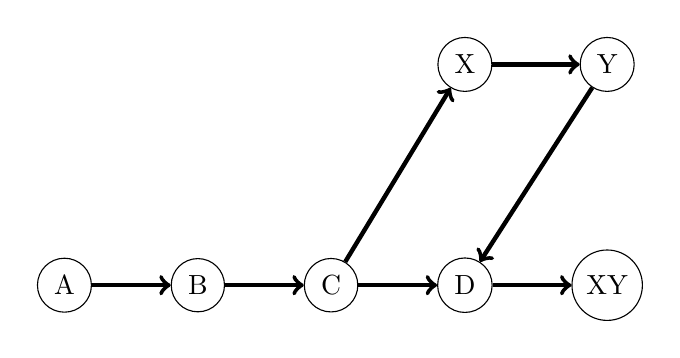
\begin{tikzpicture}
        \matrix [ampersand replacement=\&, column sep=1cm, row sep=2cm] {
            % Top
            \&
            \&
            \&
            \node (X) [draw, shape=circle, visible on=<1->] {X}; \&
            \node (Y) [draw, shape=circle, visible on=<1->] {Y}; \\
            % Bottom
            \node (A) [draw, shape=circle, visible on=<1->] {A}; \&
            \node (B) [draw, shape=circle, visible on=<1->] {B}; \&
            \node (C) [draw, shape=circle, visible on=<1->] {C}; \&
            \node (D) [draw, shape=circle, visible on=<1->] {D}; \&
            \node (XY) [draw, shape=circle, visible on=<2>] {XY}; \\
        };

        \draw[->, ultra thick] (A) -- (B);
        \draw[->, ultra thick] (B) -- (C);
        \draw[->, ultra thick, visible on=<1-2>] (C) -- (D);
        \draw[->, ultra thick] (C) -- (X);
        \draw[->, ultra thick] (X) -- (Y);
        \draw[->, ultra thick, visible on=<3>] (Y) -- (D);
        \draw[->, ultra thick, visible on=<2>] (D) -- (XY);
    \end{tikzpicture}

    \note<1>{Conflict = git doesn't know which code is 'right' \\ Here's the
    example we'll work with \\ We're on D trying to add the changes in X and Y}

    \note<2>{Merge = new commit, non-destructive}

    \note<3>{Rebase = undo, replay, redo; cleaner}
\end{frame}

\begin{frame}{Going back}
    \begin{itemize}
        \item<1->Show - look back

        \item<2->Checkout - move back

        \item<3->Reset - delete back

        \item<4->Revert - merge back
    \end{itemize}

    \note<1>{Use show to see old files}

    \note<2>{Use checkout to checkout an old commit (can make new branches)}

    \note<3>{Use reset to delete commits}

    \note<4>{Use revert to 'safe' delete commits (like merge, makes new commit)}
\end{frame}

\begin{frame}{Useful to know}
    \begin{itemize}
        \item<1->\texttt{.gitignore} - ignore non-project files

        \item<2->Decentralization

        \item<3->Merge request
    \end{itemize}

    \note<1>{Use to ignore files that change too much or are computer specific}

    \note<2>{Can push/pull directly to each other's computers if you can find
    each other on network}

    \note<3>{Used in typical work flow}
\end{frame}

\begin{frame}{Typical Workflow}
    \begin{itemize}
        \item<1->Central Repository

        \item<2->Stable Branch

        \item<3->Isolated development branches

        \item<4->Merge Request Workflow
            \begin{enumerate}
                \item<5->\texttt{git checkout -b "my\_branch"}

                \item<6->Do work...

                \item<7->\texttt{git rebase master}

                \item<8->\texttt{git push -u origin my\_branch}

                \item<9->Merge request
            \end{enumerate}
    \end{itemize}

    \note<1>{Uses a central master repo}

    \note<2>{Maintains 1 or 2 main 'stable' branches}

    \note<3>{Work is done in 'safe' branches}

    \note<4>{Merge requests are used to bring-in the changes}

    \note<5>{Sample workflow. start by making new branch}

    \note<6>{Then do whatever you need}

    \note<7>{Then rebase off the stable branch, fixing any merge conflicts now}

    \note<8>{Push the new branch up to the repo}

    \note<9>{Use repo tools to merge}
\end{frame}

\begin{frame}{Easy Mode}
    \begin{itemize}
        \item<1->Central Repository

        \item<1->Stable Branch

        \item<1->Isolated development branches

        \item<2->Just merge on master at end
    \end{itemize}

    \note<1>{Mostly the same}

    \note<2>{But at end merge directly onto master then push and say "I'm
    pushing"}
\end{frame}

\begin{frame}{Ready to try?}
    \begin{enumerate}
        \item<1->Install: git-scm.com

        \item<2->Configure:
            \begin{itemize}
                \item<2->\texttt{git config --global user.name "Your Name"}

                \item<3->\texttt{git config --global user.email "you@example.com"}
            \end{itemize}

        \item<3->Setup or Clone:
            \begin{itemize}
                \item<2->\texttt{git clone https://github.com/Labdabeta/gittut.git}
            \end{itemize}
    \end{enumerate}

    \note<1>{First you need git, get it here}

    \note<2>{Now setup who you are in git}

    \note<3>{Now start a project to track. You can use git init to make your own
    or clone mine. Just clone mine for now. (zoom in to cloning it myself in
    side terminal)}
\end{frame}

\begin{frame}{Make your change}
    \begin{enumerate}
        \item<1->Create a branch with your name (no spaces):
            \texttt{git checkout -b "john\_doe"}

        \item<2->Add your name to the users file:
            \texttt{echo "john doe" >> users.txt}

        \item<3->Stage your changes:
            \texttt{git add users.txt}

        \item<4->Commit them:
            \texttt{git commit -m "Added john doe"}

        \item<5->Rebase off of master:
            \texttt{git rebase master}

        \item<6->Push your branch:
            \texttt{git push -u origin john\_doe}
    \end{enumerate}

    \note<5>{There may be merge conflicts, just make your name last.}
\end{frame}

\begin{frame}{Unity Quirks}
    \begin{itemize}
        \item<1-> .gitignore

        \item<2-> Scenes \begin{itemize}
                \item<3-> Ignore them
                \item<4-> Resolve them
                \item<5-> Merge them
        \end{itemize}
    \end{itemize}

    \note<1>{Download .gitignore online. Easily google-able.}

    \note<2>{Scenes can't be merged by git.}

    \note<3>{Add scenes to gitignore and share manually, tedious but easy. (or
    just use separate scenes.}

    \note<4>{Use \texttt{-s theirs} or \texttt{-s ours} on merge.}

    \note<5>{Setup smart merge:
    \url{https://docs.unity3d.com/Manual/SmartMerge.html}}
\end{frame}

\iffalse
\begin{frame}{Further Reading}
    \begin{itemize}
        \item<1->Hooks

        \item<2->Issue Trackers

        \item<3->Managers (e.g. GitHub)

        \item<4->Servers

        \item<5->Mergetools / Difftools
    \end{itemize}

    \note<1>{Parting thoughts... Hooks allow you to run arbitrary programs on
    commit/checkout/push/etc}

    \note<2>{Issue trackers let you say which issue a commit fixes, often setup
    branch structure nicely}

    \note<3>{Remote repo managers like github/etc often have different
    features/costs/privacy/etc}

    \note<4>{Special servers with their own git hooks. e.g. Jenkins}

    \note<5>{Many cool merge/diff tools}
\end{frame}
\fi
\end{document}

% topics:
% git setup, .gitignore, typical workflow + game jam modification (no merge
% request, just "I'm pushing") [ as an example have audience add their names to
% a file? ]
